%\documentclass{standalone}
%\usepackage{amsmath}
%\usepackage{tikz}
%\usepackage{xcolor}
%\usetikzlibrary{fit,positioning}
%\begin{document}
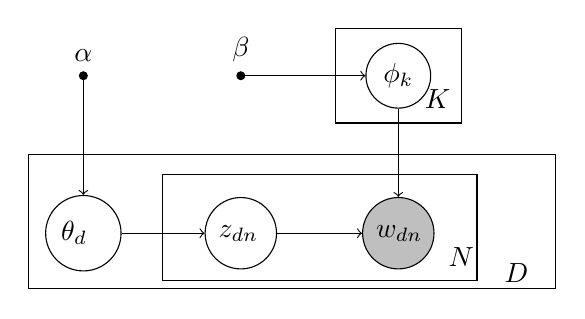
\begin{tikzpicture}
\coordinate (alpha)   at (0,2);
\node (alpha) at (0,2) [circle, draw, inner sep=1pt, fill, label=above:$\alpha$] { };
\node (theta) at (0,0) [circle, draw, text width = 16pt] {$\text{ }\theta_d$};

\node (b) at (2,2) [circle, draw, inner sep=1pt, fill, label=above:$\beta$] { };
\node (z) at (2,0) [circle, draw, text width = 16pt] {$z_{dn}$};

\node (psis) at (4,2) [circle, draw] {$\phi_k$};
\node (w) at (4,0) [circle, draw, text width = 16pt, fill=gray!50] {$w_{dn}$};

 
\draw[->] (alpha) -- (theta);
\draw[->] (b.east) -- (psis.west);
 
\draw[->] (theta.east) -- (z.west);
\draw[->] (z.east) -- (w.west);
\draw[->] (psis) -- (w);
 
\draw (-0.7,-.7) rectangle (6.,1);
\draw (1,-.6) rectangle (5,.75);
\draw (3.2,1.4) rectangle (4.8,2.6);
 
\node at (5.5,-.5) {$D$};
\node at (4.8,-.3) {$N$};
\node at (4.5,1.7) {$K$};
  
\end{tikzpicture}
%\end{document}